\documentclass[3p, authoryear, review]{elsarticle} %review=doublespace preprint=single 5p=2 column
%%% Begin My package additions %%%%%%%%%%%%%%%%%%%
\usepackage[hyphens]{url}

  \journal{Submitted to Transport Findings} % Sets Journal name


\usepackage{lineno} % add
\providecommand{\tightlist}{%
  \setlength{\itemsep}{0pt}\setlength{\parskip}{0pt}}

\usepackage{graphicx}
\usepackage{booktabs} % book-quality tables
%%%%%%%%%%%%%%%% end my additions to header

\usepackage[T1]{fontenc}
\usepackage{lmodern}
\usepackage{amssymb,amsmath}
\usepackage{ifxetex,ifluatex}
\usepackage{fixltx2e} % provides \textsubscript
% use upquote if available, for straight quotes in verbatim environments
\IfFileExists{upquote.sty}{\usepackage{upquote}}{}
\ifnum 0\ifxetex 1\fi\ifluatex 1\fi=0 % if pdftex
  \usepackage[utf8]{inputenc}
\else % if luatex or xelatex
  \usepackage{fontspec}
  \ifxetex
    \usepackage{xltxtra,xunicode}
  \fi
  \defaultfontfeatures{Mapping=tex-text,Scale=MatchLowercase}
  \newcommand{\euro}{€}
\fi
% use microtype if available
\IfFileExists{microtype.sty}{\usepackage{microtype}}{}
\usepackage{natbib}
\bibliographystyle{plainnat}
\usepackage{longtable}
\usepackage{graphicx}
% We will generate all images so they have a width \maxwidth. This means
% that they will get their normal width if they fit onto the page, but
% are scaled down if they would overflow the margins.
\makeatletter
\def\maxwidth{\ifdim\Gin@nat@width>\linewidth\linewidth
\else\Gin@nat@width\fi}
\makeatother
\let\Oldincludegraphics\includegraphics
\renewcommand{\includegraphics}[1]{\Oldincludegraphics[width=\maxwidth]{#1}}
\ifxetex
  \usepackage[setpagesize=false, % page size defined by xetex
              unicode=false, % unicode breaks when used with xetex
              xetex]{hyperref}
\else
  \usepackage[unicode=true]{hyperref}
\fi
\hypersetup{breaklinks=true,
            bookmarks=true,
            pdfauthor={},
            pdftitle={The Effect of Transit Signal Priority on Bus Rapid Transit Headway Adherence},
            colorlinks=false,
            urlcolor=blue,
            linkcolor=magenta,
            pdfborder={0 0 0}}
\urlstyle{same}  % don't use monospace font for urls

\setcounter{secnumdepth}{5}
% Pandoc toggle for numbering sections (defaults to be off)


% Pandoc header
\usepackage{booktabs}
\usepackage{booktabs}
\usepackage{longtable}
\usepackage{array}
\usepackage{multirow}
\usepackage{wrapfig}
\usepackage{float}
\usepackage{colortbl}
\usepackage{pdflscape}
\usepackage{tabu}
\usepackage{threeparttable}
\usepackage{threeparttablex}
\usepackage[normalem]{ulem}
\usepackage{makecell}
\usepackage{xcolor}



\begin{document}
\begin{frontmatter}

  \title{The Effect of Transit Signal Priority on Bus Rapid Transit Headway Adherence}
    \author[BYU]{Gregory Macfarlane\corref{1}}
   \ead{gregmacfarlane@byu.edu} 
    \author[BYU]{Grant Schultz}
   \ead{gschultz@byu.edu} 
    \author[WCG]{Michael Sheffield}
   \ead{michael.sheffield@wcg.us} 
    \author[BYU]{Logan Bennett}
   \ead{loganbennett93@gmail.com} 
      \address[BYU]{Brigham Young University, Civil and Environmental Engineering Department, 430 Engineering Building, Provo, Utah 84602}
    \address[WCG]{Wall Consultant Group, 9980 S 300 W Ste 200 Sandy, UT 84070}
      \cortext[1]{Corresponding Author}
  
  \begin{abstract}
  We report the results of an experiment to evaluate the impact of transit signal priority (TSP) on headway adherence for a bus rapid transit (BRT) system in Provo / Orem, Utah. The bus requests TSP based on its unpublished schedule, but users perceive only a headway. Quantile regression models estimated on raw timepoint data from the BRT system reveal that TSP significantly improves headway adherence, after controlling for peak times, direction, and cumulative trip dwell time. We also find that requiring the bus to be 2 minutes late before requesting TSP improves headway adherence more than allowing all buses to request TSP.
  \end{abstract}
   \begin{keyword} Public transit, Transit signal priority, Traffic operations\end{keyword}
 \end{frontmatter}

\hypertarget{intro}{%
\section{Questions}\label{intro}}

Transit signal priority (TSP) allows traffic signals to flexibly accommodate
transit vehicles. This may involve extending a green phase until the vehicle
passes, triggering an early green if there is a vehicle waiting at the light, or
even running specific transit-only phases. TSP helps transit vehicles maintain
on-time performance \citep{sheffieldsensitivity, Liu2018}, but often TSP will only engage at a signal if
the vehicle is running behind its schedule, thus minimizing automobile delay
when the bus is otherwise on schedule \citep{NI20201}.

In 2018, the Utah Transit Authority (UTA) launched the Utah Valley Express (UVX)
Bus Rapid Transit (BRT) system in Provo and Orem, Utah. The system connects
two commuter rail stations, two major universities (Brigham Young and Utah Valley),
and commercial districts in Orem and Provo. UVX has TSP on 44 of the 47 traffic
signals along its route. A transit vehicle requests TSP the vehicle is behind its
schedule; the signal controller may then grant the TSP based on a set of rules.
For example, the signal will not grant TSP to transit vehicles traveling in the
same direction in consecutive signal cycles. Specifically, at least two ``clean'' cycles
must run before the signal controller will grant TSP again.

Though the TSP system is based on a schedule, UTA does not publish a schedule
for UVX. Instead informed that a bus will arrive on a specific
headway: 6 minutes in the peak period and 10 minutes in the off-peak. UVX vehicles depart
their initial time point on this schedule, but then proceed to the end of the route
without consideration as to whether the vehicle is running ahead or behind its ``schedule''
as understood by the TSP system. It is
unclear whether the actualized headway is affected by a schedule-based TSP
system, potentially creating frustration for riders or inefficient operations.
The research questions are therefore:

\begin{itemize}
\tightlist
\item
  Does schedule-based TSP improve headway adherence for rapid transit systems?
\item
  What other factors influence headway adherence: direction, dwell time, etc.?
\end{itemize}

\hypertarget{methods}{%
\section{Methods}\label{methods}}

UTA provided time point data for all trips on the UVX system for the entirety of
2019. We calculated the headway between successive UVX trips at each stop, as
well as the cumulative dwell time of all stations along the route to that point.
Because the UVX route loops around south Provo and stops at the Provo
FrontRunner station twice, this created some minor difficulties in data
processing, and we removed the time points on this portion of the route. We also
limit our analysis to the periods between 7 AM and 8 PM when the system runs at
a 6-minute headway. Time points within these periods are considered ``AM Peak'' if
occurring between 7 and 9 AM, or ``PM Peak'' between 4 and 6 PM.

From January through June 6, the system operated with a 5-minute TSP request
threshold due to an erroneous system configuration; these time points were
discarded. After August 12, the system switched to a 2-minute TSP request
threshold. During the summer, the TSP system was configured as follows for this
experiment:

\begin{itemize}
\tightlist
\item
  June 10 through July 12 and after August 12: 2 minute threshold
\item
  July 15 through July 26: no TSP
\item
  July 30 through August 9: TSP always requested
\end{itemize}

We also discarded trips from January through April and September through
December because the additional university passenger demand could interfere in
the experiment and there were no tests of the ``None'' or ``Always'' TSP thresholds
during the school year.

Standard statistical tests --- such as the student's \(t\)-test or
ordinary least squares regression models --- are designed to ascertain the
significance of a statistic at the \emph{mean} of the distribution. In this
application, we are less concerned with the mean deviation in headway, and are
instead interested in whether TSP is able to reduce the lateness of buses that
already have substantial deviation from their programmed headway. Further, a bus
that is delayed from its intended headway may shorten the subsequent headway due
to ``bunching.'' Consequently, we employ conditional quantile regression
\citep{koenker2001quantile} to estimate the effect of TSP requesting threshold on
headway deviation at multiple percentiles of the distribution. This is
done with the \texttt{quantreg} package for R \citep{quantreg, R}

\hypertarget{findings}{%
\section{Findings}\label{findings}}

Figure \ref{fig:ecdf} shows the empirical cumulative density function for the
headway deviation data, grouped by TSP threshold. Note that a ``perfect''
headway distribution, where all vehicles maintain the exactly intended headway,
would be step function with a vertical transition at six minutes.
Visually, the difference between the various threshold settings is not dramatic.
The 2-minute threshold appears to have slightly more vehicles arrive behind the
scheduled headway (6 minutes), and slightly more arrive before it, than the
other two threshold groups. The median of the distribution for all
four thresholds is remarkably similar and is just a few seconds behind the target
headway. This observation strengthens our determination to examine the sides of
the distribution --- rather than its center --- with a quantile regression model.

\begin{figure}
\centering
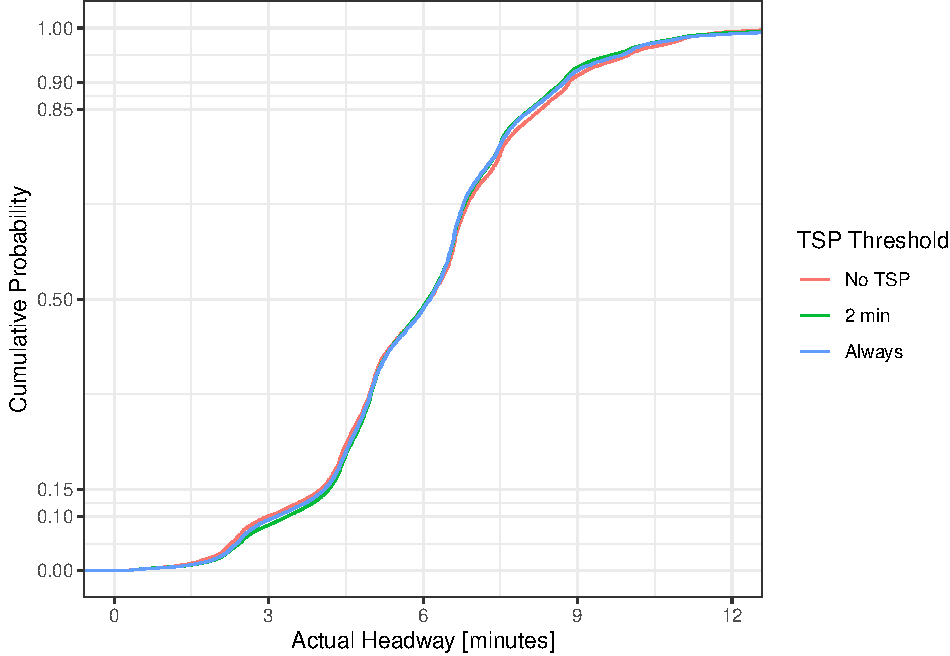
\includegraphics{uvx_headways_files/figure-latex/ecdf-1.pdf}
\caption{\label{fig:ecdf}Cumulative probability distribution of headway deviation by threshold.}
\end{figure}

Models estimating the headway effects of TSP requesting threshold and other factors
at an array of distribution quantiles are given in Table \ref{tab:models-summ}.
In these models, the ``(Intercept)'' represents the expected headway at that percentile
before considering additional information. For example, the 10th-percentile headway
is 4.649 minutes, all else equal. The other
coefficients in the models modify this average headway. Almost all coefficients are
significant, and many serve to widen the headway distribution.
Buses traveling in the PM peak, for example, have a significantly higher
90th-percentile headway and a lower 10th-percentile headway. Buses traveling in the
southbound direction also have a wider headway distribution than those in the
northbound direction, and an additional minute of cumulative dwell time widens the
the headway distribution.

\begin{landscape}\begin{table}

\caption{\label{tab:models-summ}Quantile Regression Estimates}
\centering
\resizebox{\linewidth}{!}{
\begin{tabular}[t]{lccccc}
\toprule
  & 10th & 15th & 50th & 85th & 90th\\
\midrule
(Intercept) & 4.649 (108.947)*** & 4.922 (131.183)*** & 6.338 (174.147)*** & 7.410 (187.349)*** & 7.598 (209.077)***\\
TSP: 2 minutes & 0.190 (5.234)*** & 0.168 (4.880)*** & -0.013 (-0.400) & -0.186 (-5.346)*** & -0.178 (-5.399)***\\
TSP: Always & 0.093 (2.033)** & 0.101 (2.479)** & 0.001 (0.018) & -0.218 (-4.650)*** & -0.132 (-2.835)***\\
Southbound & -0.921 (-21.746)*** & -0.604 (-17.391)*** & -0.161 (-4.591)*** & 0.752 (21.580)*** & 0.861 (26.837)***\\
AM Peak & -0.160 (-5.148)*** & -0.114 (-3.578)*** & 0.075 (2.973)*** & -0.068 (-1.211) & 0.112 (3.453)***\\
PM Peak & -0.444 (-8.855)*** & -0.204 (-4.895)*** & -0.401 (-6.218)*** & 0.380 (9.390)*** & 0.461 (12.282)***\\
Cumulative Dwell [minutes] & -0.205 (-44.282)*** & -0.175 (-33.066)*** & -0.041 (-8.505)*** & 0.105 (15.956)*** & 0.161 (31.324)***\\
Southbound $\times$ AM Peak & 0.004 (0.063) & -0.067 (-1.144) & 0.141 (2.876)*** & 0.415 (6.201)*** & 0.257 (4.611)***\\
Southbound $\times$ PM Peak & 0.285 (4.076)*** & -0.286 (-5.420)*** & -0.003 (-0.032) & -0.171 (-2.371)** & -0.157 (-2.470)**\\
\midrule
AIC & 321,907.1 & 314,210.7 & 301,346.1 & 325,312.4 & 336,009.8\\
Log Likelihood & -160,944.5 & -157,096.3 & -150,664 & -162,647.2 & -167,995.9\\
\bottomrule
\multicolumn{6}{l}{\textsuperscript{} t-statistics in parentheses, * p $<$ 0.1, ** p $<$ 0.05, *** p $<$ 0.01}\\
\multicolumn{6}{l}{\textsuperscript{} Coefficients represent change to expected headway in minutes.}\\
\end{tabular}}
\end{table}
\end{landscape}

In contrast, the estimates reveal that TSP significantly
\emph{narrows} the expected headway distribution, with fewer long headways and fewer
short headways. And while most of the other explanatory variables have
an effect on the median headway, TSP has no significant effect after these other
variables have been controlled for.
A potentially curious finding is that implementing a 2-minute TSP request
threshold improves headway adherence more than allowing every transit vehicle to
request TSP. This could be an artifact of the signal controller not
granting requests in consecutive cycles, or it could be that always requesting TSP
exacerbates bunching.

The schedule of threshold changes was not randomized in any way,
and it is possible that the results of this study are tied up in unaccounted
seasonal variation, or other omitted explanatory variables. These limitations
notwithstanding, we find that --- all else equal --- TSP marginally improves the
headway adherence of UVX.

\bibliography{book.bib}


\end{document}

